% !TeX spellcheck = es_ES
% Chapter 1

%\chapter{Chapter Title Here} % Main chapter title
%
%\label{Chapter1} % For referencing the chapter elsewhere, use \ref{Chapter1} 

%----------------------------------------------------------------------------------------

% Define some commands to keep the formatting separated from the content 
%\newcommand{\keyword}[1]{\textit{#1}}
%\newcommand{\tabhead}[1]{\textbf{#1}}
%\newcommand{\code}[1]{\texttt{#1}}
%\newcommand{\file}[1]{\texttt{\bfseries#1}}
%\newcommand{\option}[1]{\texttt{\itshape#1}}

%----------------------------------------------------------------------------------------

\chapter{Calibraci\'on Qu\'imica}
	La calibraci\'on qu\'imica consiste en contrastar las propiedades termodin\'amicas de un sistema qu\'imico, obtenidas usando el calor\'imetro con aquellas reportadas en la literatura. Para esto se estudia la reacci\'on del \'acido clorhidrico con bicarbonato de potasio. Esta reacci\'on presenta varias ventajas: por un lado hace uso de reactivos de f\'acil acceso, es una reacci\'on con esqueometr\'ia 1:1, ha sido estudiada previamente, y adem\'as, es usada en calibraciones de equipos calorim\'etricos., como el calor\'imetro de titulaci\'on NanoITC de \textit{TA instruments}.
	
\section{Preparaci\'on de las soluciones de HCl}\label{sec: soluciones}
	Para la preparaci\'on de las soluciones, se hace uso de forma sistem\'atica de una balanza Ohaus Analytical Plus (AP250D) y un dens\'imetro Anton Paar DSA5000M. La balanza presenta incertidumbres de $1\times10^{-5}$ y $1\times10^{-4}$ g dependiendo del rango usado, para el primer caso la masa medida debe ser inferior a 80 g y en el segundo no puede superar los 250 g, siendo esta la capacidad máxima de la balanza. En el caso del densímetro, son necesarios volúmenes cercanos a 2 mL de una muestra líquida, con esto el equipo determina la densidad de la sustancia con incertidumbres de $1\times10^{-6}$ g/cm$^{-3}$ para una temperatura determinada por el usuario. Adem\'as, en el proceso de preparaci\'on se hace necesaria la toma de dos al\'icuotas de 30 $\mu$L y 170 $\mu$L, para el HCl y \ce{KHCO3} correspondientemente, por lo cual se usa una micropipeta pipet4u Performance con rango de 20 a 200 $\mu$L.
	
	\subsection{Soluci\'on de HCl 0.25 mM}
		Para determinar la concentraci\'on de una soluci\'on de 1,0 mL de HCl concentrado en 25,0 mL de agua tipo 1, se midi\'o la densidad de la soluci\'on, posteriormente usando como referencia los datos reportados en la literatura fue realizada una regresi\'on lineal que permiti\'o relacionar la concentraci\'on con la densidad de la soluci\'on $\rho$ \cite{perry2007perry}. De esta manera se estableci\'o el valor de la concentraci\'on en: $3.02 \pm 0.05$ \% (fracci\'on de masa $[w_t]$), donde la incertidumbre se obtiene de la pendiente ($m$) e intercepto ($b$) de la regresi\'on lineal que se muestra en la \autoref{fig: HCl_density}.
		\begin{equation}
			\delta [w_t] = \sqrt{\left(\dfrac{\rho-b}{m^2}\delta m\right)^2 + \left(\dfrac{\delta b}{m}\right)^2 + \left(\dfrac{\delta \rho}{m}\right)^2}
		\end{equation}
		\begin{figure}[h]
			\centering
			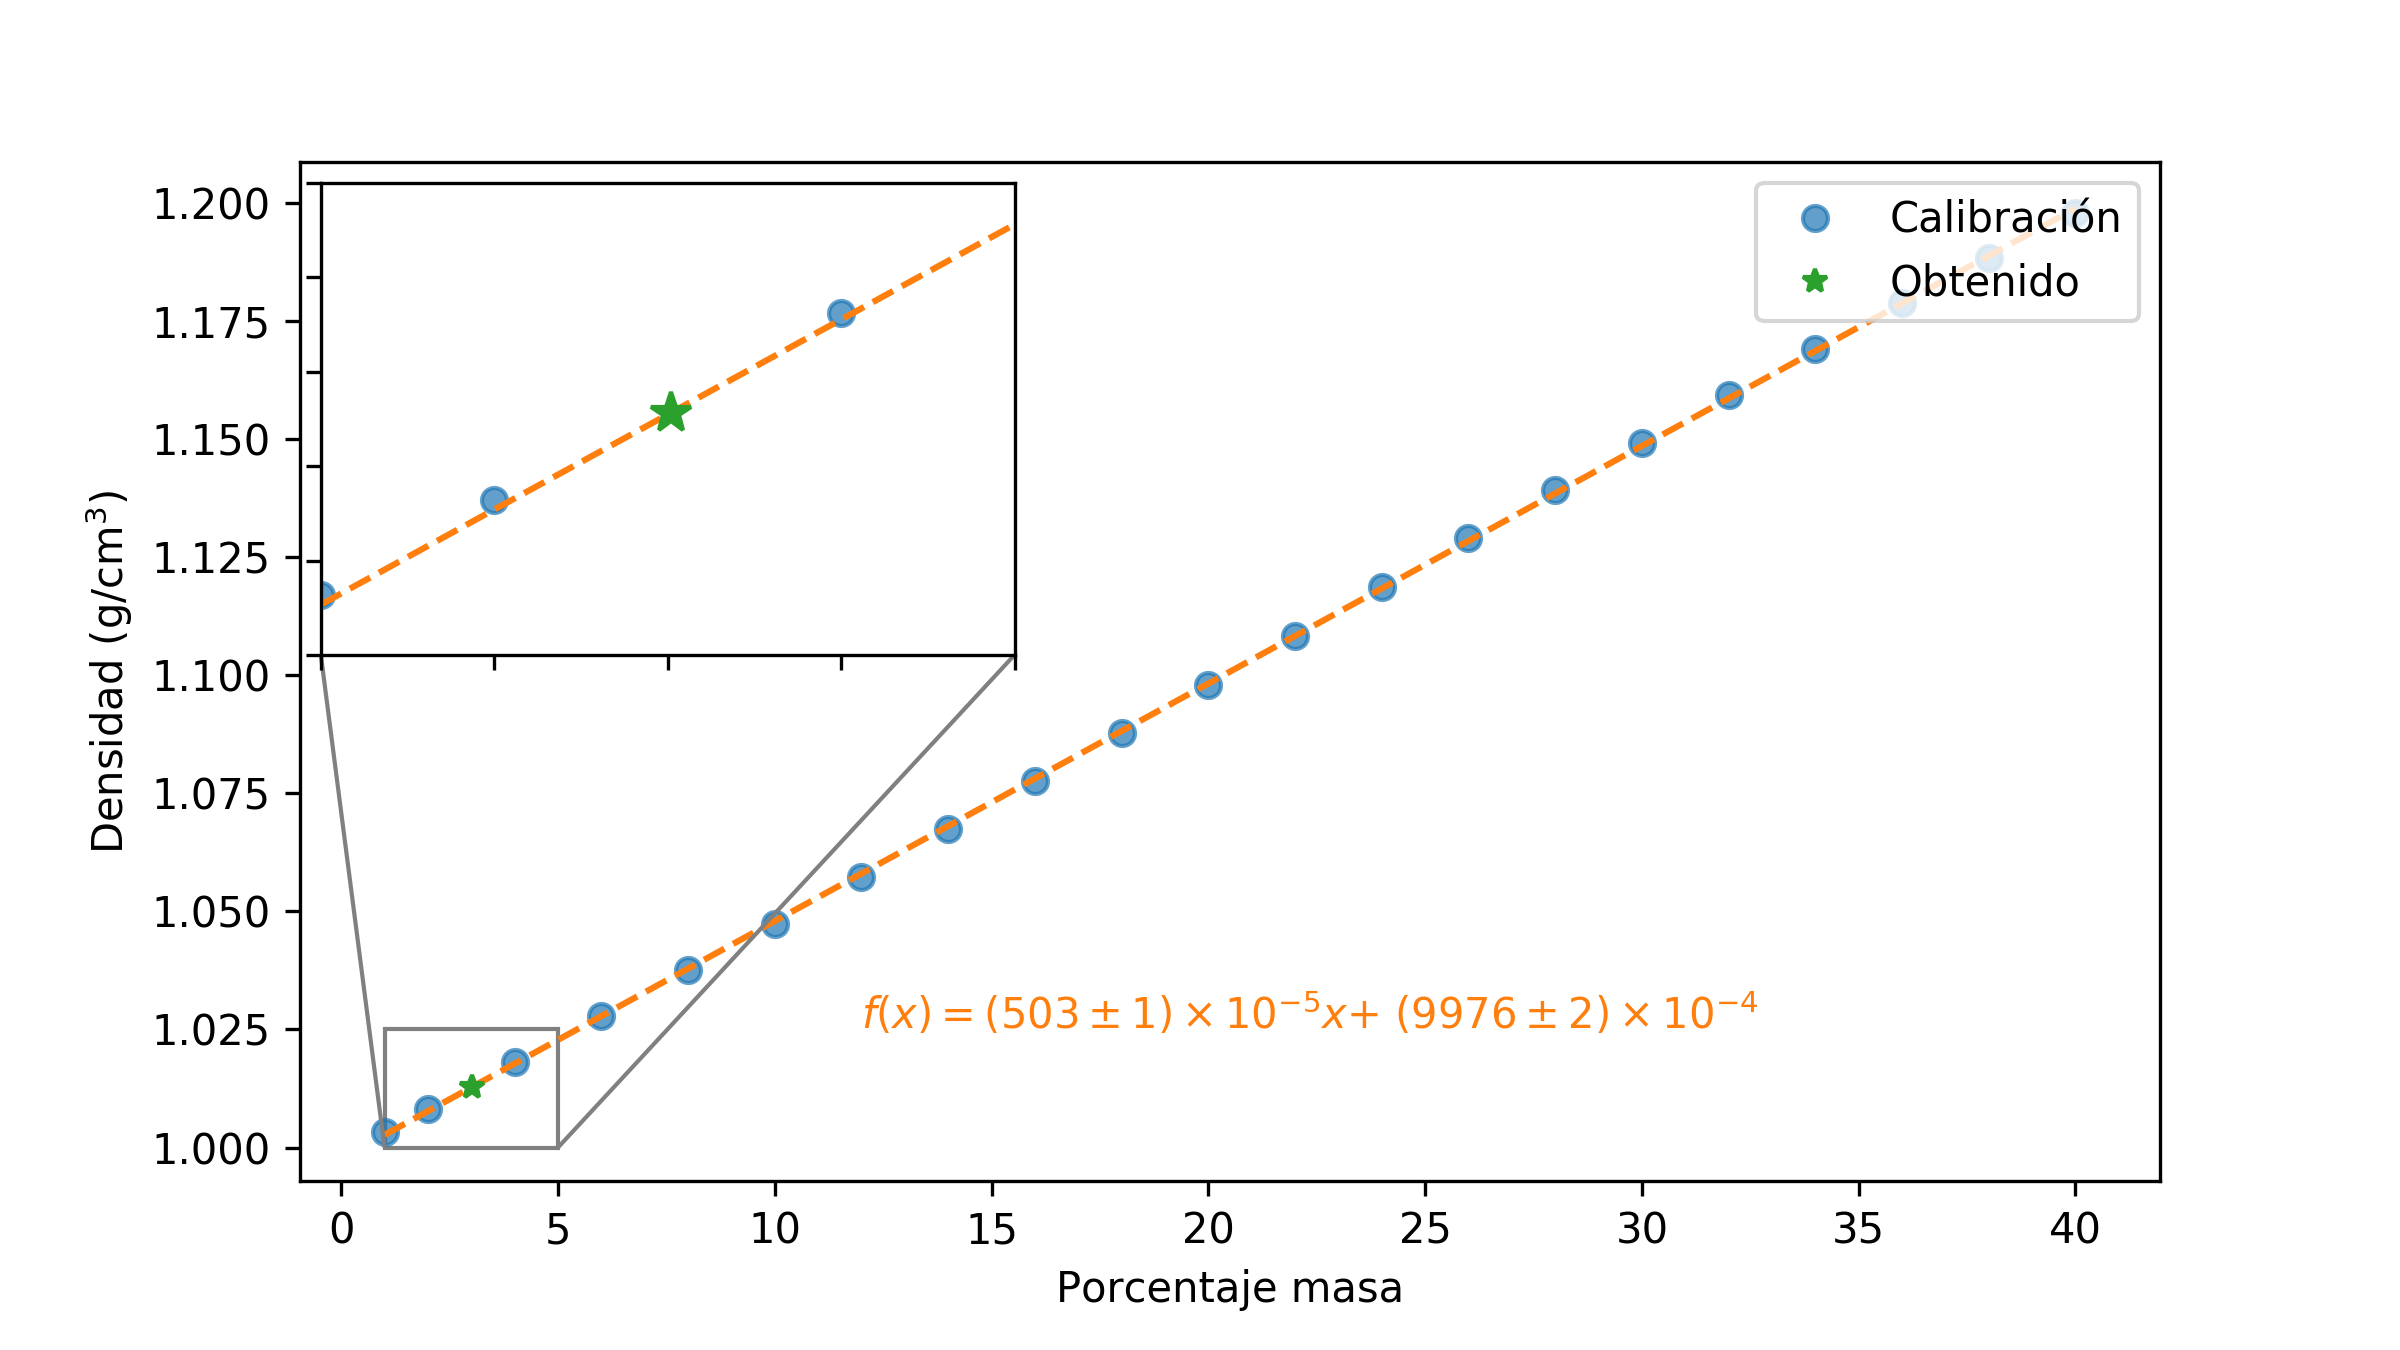
\includegraphics[width=\linewidth]{../Data/Concentration/C_HCl_initial.png}
			\caption{Determinaci\'on de la concentraci\'on de una soluci\'on de HCl usando valores de densidad reportados en la literatura \cite{perry2007perry}.}
			\label{fig: HCl_density}
		\end{figure}
		
		Para obtener la concentraci\'on $0.84 \pm 0.04$ M, se usa la siguiente ecuaci\'on, la cual relaciona la concentraci\'on en fracci\'on de masa con la molaridad $[M]$:
		\begin{equation}
			[M] = 10\dfrac{[w_t]\rho}{m_m} \qquad \text{$m_m$ la masa molecular del HCl}
		\end{equation}
		
		Se tiene entonces que la incertidumbre en la concentraci\'on estar\'a dada por:
		\begin{equation}
			\delta [M] = [M]\sqrt{\delta[w_t]^2 + \delta\rho^2} 
		\end{equation}
		
		Una al\'icuota de 0,0297 g de esta soluci\'on fue disuelta en 99,5553 g de agua, dando lugar a una soluci\'on 0,2469 mM. Donde la concentraci\'on final se calcula a partir de las densidades de las soluciones inicial ($\rho_s$) y final ($\rho_f$), las masas de agua ($m_\text{\ce{H2O}}$) y de soluci\'on inicial ($m_s$) usando la siguiente ecuaci\'on:
		\begin{equation}\label{eq: concentracion_f}
			[M]_f = [M]_i\dfrac{V_s}{V_f} = [M_i]\dfrac{m_s/\rho_s}{(m_s + m_{\text{\ce{H2O}}})/\rho_f} =  [M]_i\left(\dfrac{m_s}{m_s + m_{\text{\ce{H2O}}}}\right)\left(\dfrac{\rho_s}{\rho_f}\right)
		\end{equation}
		
		Las densidades de las soluciones inicial y final se muestran en la \autoref{tb: concentracion_f}.
		
	\subsection{Soluci\'on de \ce{KHCO3} 0.17 mM}
	En un bal\'on aforado de 10 mL fueron adicionados 0,10143 g de \ce{KHCO3}, junto con 9,93551 g de \ce{H2O}. La densidad fue medida a 25 $^\circ$C y su valor fue 1,003662 g/cm$^3$. La concentraci\'on de esta soluci\'on se calcul\'o usando la siguiente ecuaci\'on:
	\begin{equation}
		[M] = \dfrac{n}{V} = \dfrac{m\rho}{m_m(m + m_{\ce{H2O}})}
	\end{equation}

	Obteniendo un valor de $0.10131\pm 0.00001$ M, donde la incertidumbre se calcula usando:
	\small
	\begin{equation}
		\delta[M] = \sqrt{\frac{m^{2}}{m_m^{2} \left(m + m_{\text{\ce{H2O}}}\right)^{2}}\delta\rho^{2} + \frac{\rho^{2} m_{\text{\ce{H2O}}}^{2}}{m_m^{2} \left(m + m_{\text{\ce{H2O}}}\right)^{4}}\delta m^{2} + \frac{\rho^{2} m^{2}}{m_m^{2} \left(m + m_{\text{\ce{H2O}}}\right)^{4}}\delta{m_{\text{\ce{H2O}}}}^{2}}
	\end{equation}
	\normalsize
	
	Posteriormente se tom\'o una al\'icuota de 0,1709 g, la cual fue dilu\'ida en 99,5657 g de agua. Usando la \autoref{eq: concentracion_f}, se obtiene una concentraci\'on de 0,17265 mM. El resumen de las cantidades usadas para la diluci\'on de las soluciones de \'acido y bicarbonato, as\'i como las densidades obtenidas a 20 $^\circ$C se muestran en la \autoref{tb: concentracion_f}.
	\begin{table}[h]
		\centering
		\caption{Densidades y masas medidas para preparar las soluciones con concentraciones 0,25 mM y 0,17 mM para el HCl y \ce{KHCO3} correspondientemente.}
		\small
		\begin{tabular}{c|cccccc}
			\hline
			& $\mathbf{[M]_i}$ (M) & $\mathbf{m_s}$ (g) & $\mathbf{m_{\text{H2O}}}$ (g) & $\bm{\rho_s}$ (g/cm$^3$)& $\bm{\rho_f}$ (g/cm$^3$) & $\mathbf{[M]_f}$ (mM) \\
			\hline
			\textbf{\ce{HCl}} & $0.84 \pm 0.04$ & $0.0297$ & $99.5553$ & $1.012832$ & $0.998205$ & $0.25$ \\
			\textbf{\ce{KHCO3}} & $0.10131\pm 0.00001$ & $0.1709$ & $99.5657$ & $1.003662$ & $0.998215$ & $0.17265$ \\
			\hline
		\end{tabular}
		\label{tb: concentracion_f}
	\end{table}
	
\section{Sistema de inyecci\'on}
	El sistema de inyecci\'on consiste en un motor de pasos acoplado a un tornillo de precisión, el cual controla el desplazamiento del émbolo de la jeringa de inyección. El fluido saliente de la jeringa se desvía usando una manguera de cromatografía líquida de acero inoxidable, el cual se conecta en el otro extremo a un canal que lleva el fluido hasta la celda de medición.
	
	\begin{figure}[h]
		\centering
		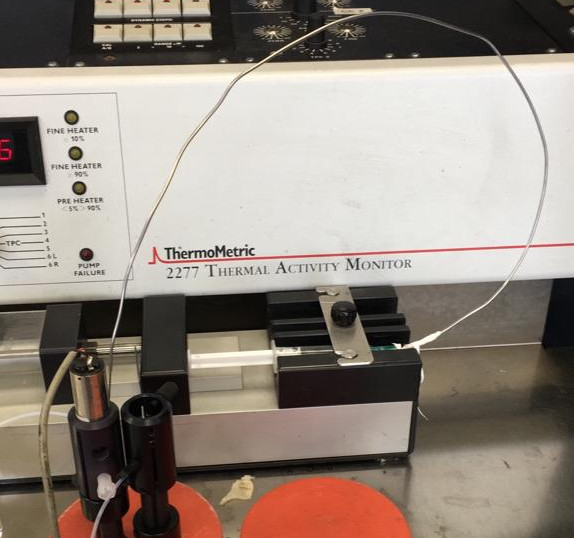
\includegraphics[width=0.5\linewidth]{Figures/sistemaInyeccion}
			
		\caption{Sistema de inyección construido como alternativa al uso de las canulas.}
		\label{fig: sistemaInyeccion}
	\end{figure}
	
	Tanto la aguja de la jeringa como la manguera de cromatografía, corresponden con una alternativa para ingresar el fluido hasta la celda que difiere del mecanismo original en los volúmenes usados y el tipo de jeringas. Originalmente, para introducir una sustancia en la celda se hace uso de una jeringa de vidrio Hammilton de 250 $\mu$L la cual cuenta con una canula soldada en la punta de esta. Al momento de realizar el experimento, no se contaba con una jeringa de este tipo con la canula conectada, y a pesar que varios intentos fueron realizados para soldar la punta con la canula de oro y acero inoxidable no fue posible juntar las partes, en parte dado que el diámetro de la canula es considerablemente pequeño, siendo difícil de ver a simple vista. Lo anterior tiene consideraciones especiales, pues los diámetros de la jeringa y la manguera no son compatibles, por lo cual se hace necesario usar cinta de teflón para evitar al máximo fugas en el sistema. Además el volumen interno de la manguera cromatogr\'afica es mucho mayor al de la canula, por lo cual se debe tener especial cuidado por los volúmenes introducidos, pues no se debe exceder la capacidad de 4 mL de la celda.
	
	\subsection{Control por software}
	Para acceder al control de la jeringa, en el menú superior: \texttt{System > Auxiliary > Pump}. En el momento se cuenta con un único agitador para la celda, por lo cual sólo se encuentra instalado uno de los controladores de jeringa tipo \texttt{Lund}, por esta razón el sistema debe detectar automáticamente únicamente el primer controlador (\texttt{Installed = yes}). La configuración de una jeringa consiste en escribir el volumen de esta (\texttt{Syringe volume}), la velocidad con la que se quiere mover el émbolo (\texttt{Plunger speed}), su longitud (\texttt{Syringe length}) y el volumen por inyección (\texttt{Dispense volume}).
	
	\begin{figure}[h]
		\centering
		\begin{subfigure}[b]{0.4\textwidth}
			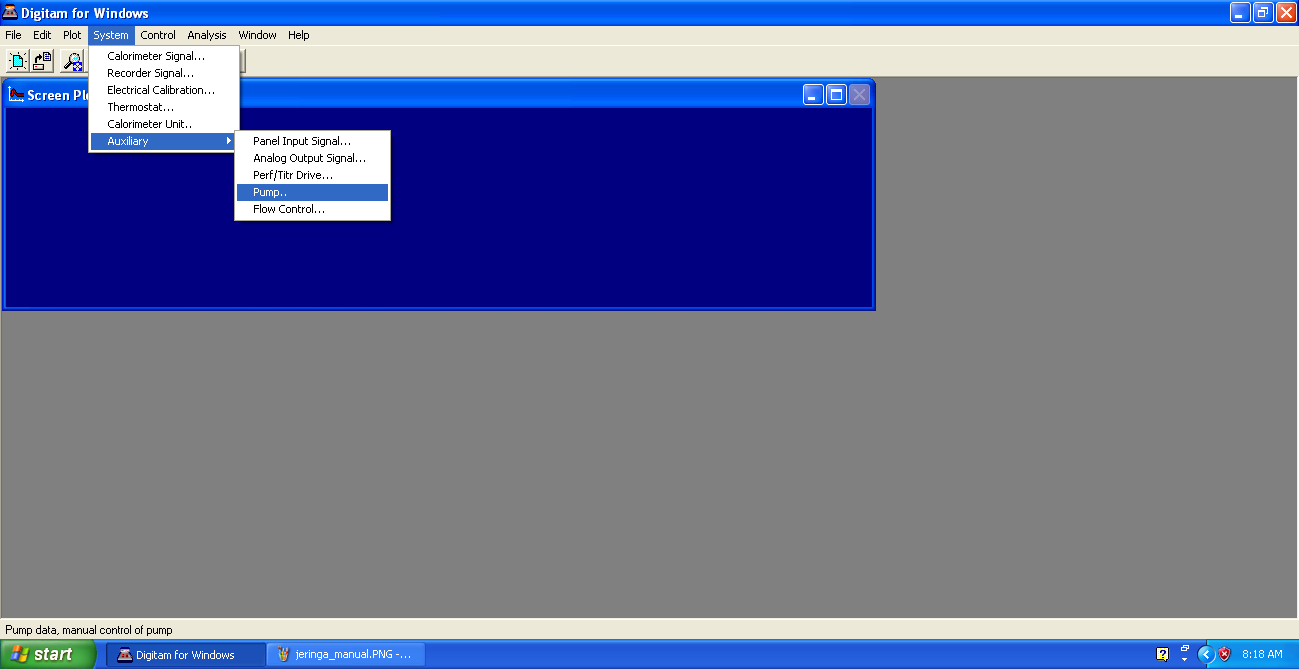
\includegraphics[width=\linewidth]{Figures/jeringa_menu}
			\caption{Ingreso al menú.}
			\label{fig: menuJeringa}
		\end{subfigure}
		\begin{subfigure}[b]{0.55\textwidth}
			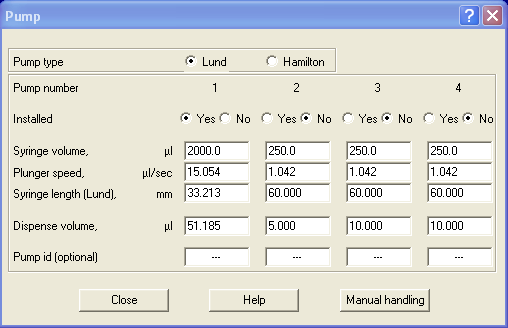
\includegraphics[width=\linewidth]{Figures/jeringa_config}
			\caption{Menú de configuración}
			\label{fig: configJeringa}
		\end{subfigure}
		\caption{Configuración de la jeringa en Digitam.}
	\end{figure}
	
	Una vez se encuentra configurada la jeringa, es posible usarla de dos maneras distintas. Por un lado se tiene el modo manual, donde el usuario tiene la posibilidad de avanzar rápidamente (\texttt{Fast forward}), por ejemplo para disminuir al distancia entre el émbolo y el pistón. También es posible aumentar esta distancia (\texttt{Fast backward}), avanzar un milímetro (\texttt{One milimeter forward}) y moverse la distancia requerida para que la jeringa dispense el volumen por inyección (\texttt{Dispense}). El control manual resulta útil antes de iniciar un experimento, pues con frecuencia será necesario ajustar la distancia entre el pistón y el émbolo para que haya contacto. Además en el caso de ser requerida una calibración de la jeringa es posible usar el botón de dispensar para determinar si el volumen dispensado corresponde con el volumen configurado.
	\begin{figure}[h]
		\centering
		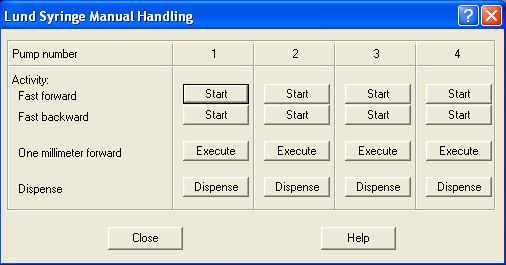
\includegraphics[width=0.5\linewidth]{Figures/jeringa_manual}
		\caption{Panel del uso manual del controlador de la jeringa.}
		\label{fig: manualJeringa}
	\end{figure}

	El modo automático se configura al momento de definir el método del experimento. Para esto es necesario expandir la opción de \texttt{Auxiliary system} en el panel izquierdo del menú y seleccionar ítem \texttt{Pump and flow control}. Se debe tener en cuenta la sección del experimento que se está configurando. En el caso de la \autoref{fig: autoJeringa}, sólo existe la sección de \texttt{Baseline}, en esta sección se busca realizar 20 inyecciones cada una con el volumen de dispensación y velocidad configurados en la \autoref{fig: configJeringa} y 300 segundos de espera entre cada inyección.
	\begin{figure}[h]
		\centering
		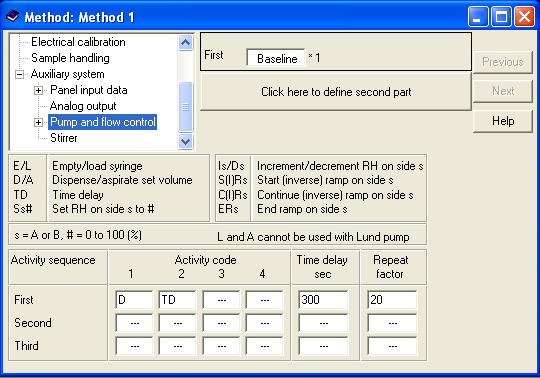
\includegraphics[width=0.5\linewidth]{Figures/jeringa_experimento}
		\caption{Panel de configuración de la jeringa en modo automático.}
		\label{fig: autoJeringa}
	\end{figure}
	
	\subsection{Calibraci\'on de la jeringa}
		Si bien el volumen de una jeringa es bien conocido, la longitud del émbolo es un parámetro que con frecuencia no se encuentra fácilmente. El controlador de la jeringa depende de este valor para relacionar la longitud que debe expandir el pistón para dispensar el volumen $V_d$. Por esta razón, para determinar la longitud correcta de la jeringa que debe ser configurada, se usaron distintos valores de esta y se midió la masa de agua tipo 1 desplazada, para cada valor de longitud se tomaron 3 medidas, los cuales se muestran en la \autoref{tb: syringeCal}.
		\begin{table}[h]
			\centering
			\caption{Masa dispensada por la jeringa usando diferentes longitudes y un $V_d = 100.000$ $\mu$L}
			\small
			\begin{tabular}{p{1.7cm}|p{1.3cm}p{1.3cm}p{1.3cm}|p{2cm}p{2cm}}
				\hline
				\textbf{Longitud (mm)} &  \textbf{Masa 1 (g)} &  \textbf{Masa 2} (g) &  \textbf{Masa 3 (g)} &  \textbf{Promedio (g)} & \textbf{Desviacion (g)} \\
				\hline
				28,000 & 0,08194 & 0,08196 & 0,08262 & 0,0822 & 0,0004 \\
				29,000 & 0,08573 & 0,08673 & 0,08648 & 0,0863 & 0,0005 \\
				30,000 & 0,09003 & 0,08884 & 0,08970 & 0,0895 & 0,0006 \\
				31,000 & 0,09270 & 0,09322 & 0,09263 & 0,0928 & 0,0003 \\
				32,000 & 0,09551 & 0,09536 & 0,09538 & 0,0954 & 0,0001 \\
				33,000 & 0,09895 & 0,09825 & 0,09870 & 0,0986 & 0,0004 \\
				34,000 & 0,10172 & 0,10176 & 0,10137 & 0,1016 & 0,0002 \\
				35,000 & 0,10409 & 0,10318 & 0,10422 & 0,1038 & 0,0006 \\
				36,000 & 0,10679 & 0,10593 & 0,10757 & 0,1068 & 0,0008 \\
				37,000 & 0,10958 & 0,11015 & 0,10993 & 0,1099 & 0,0003 \\
				38,000 & 0,11384 & 0,11327 & 0,11360 & 0,1136 & 0,0003 \\
				\hline
			\end{tabular}
			\label{tb: syringeCal}
		\end{table}
		
		\begin{figure}[h]
			\centering
			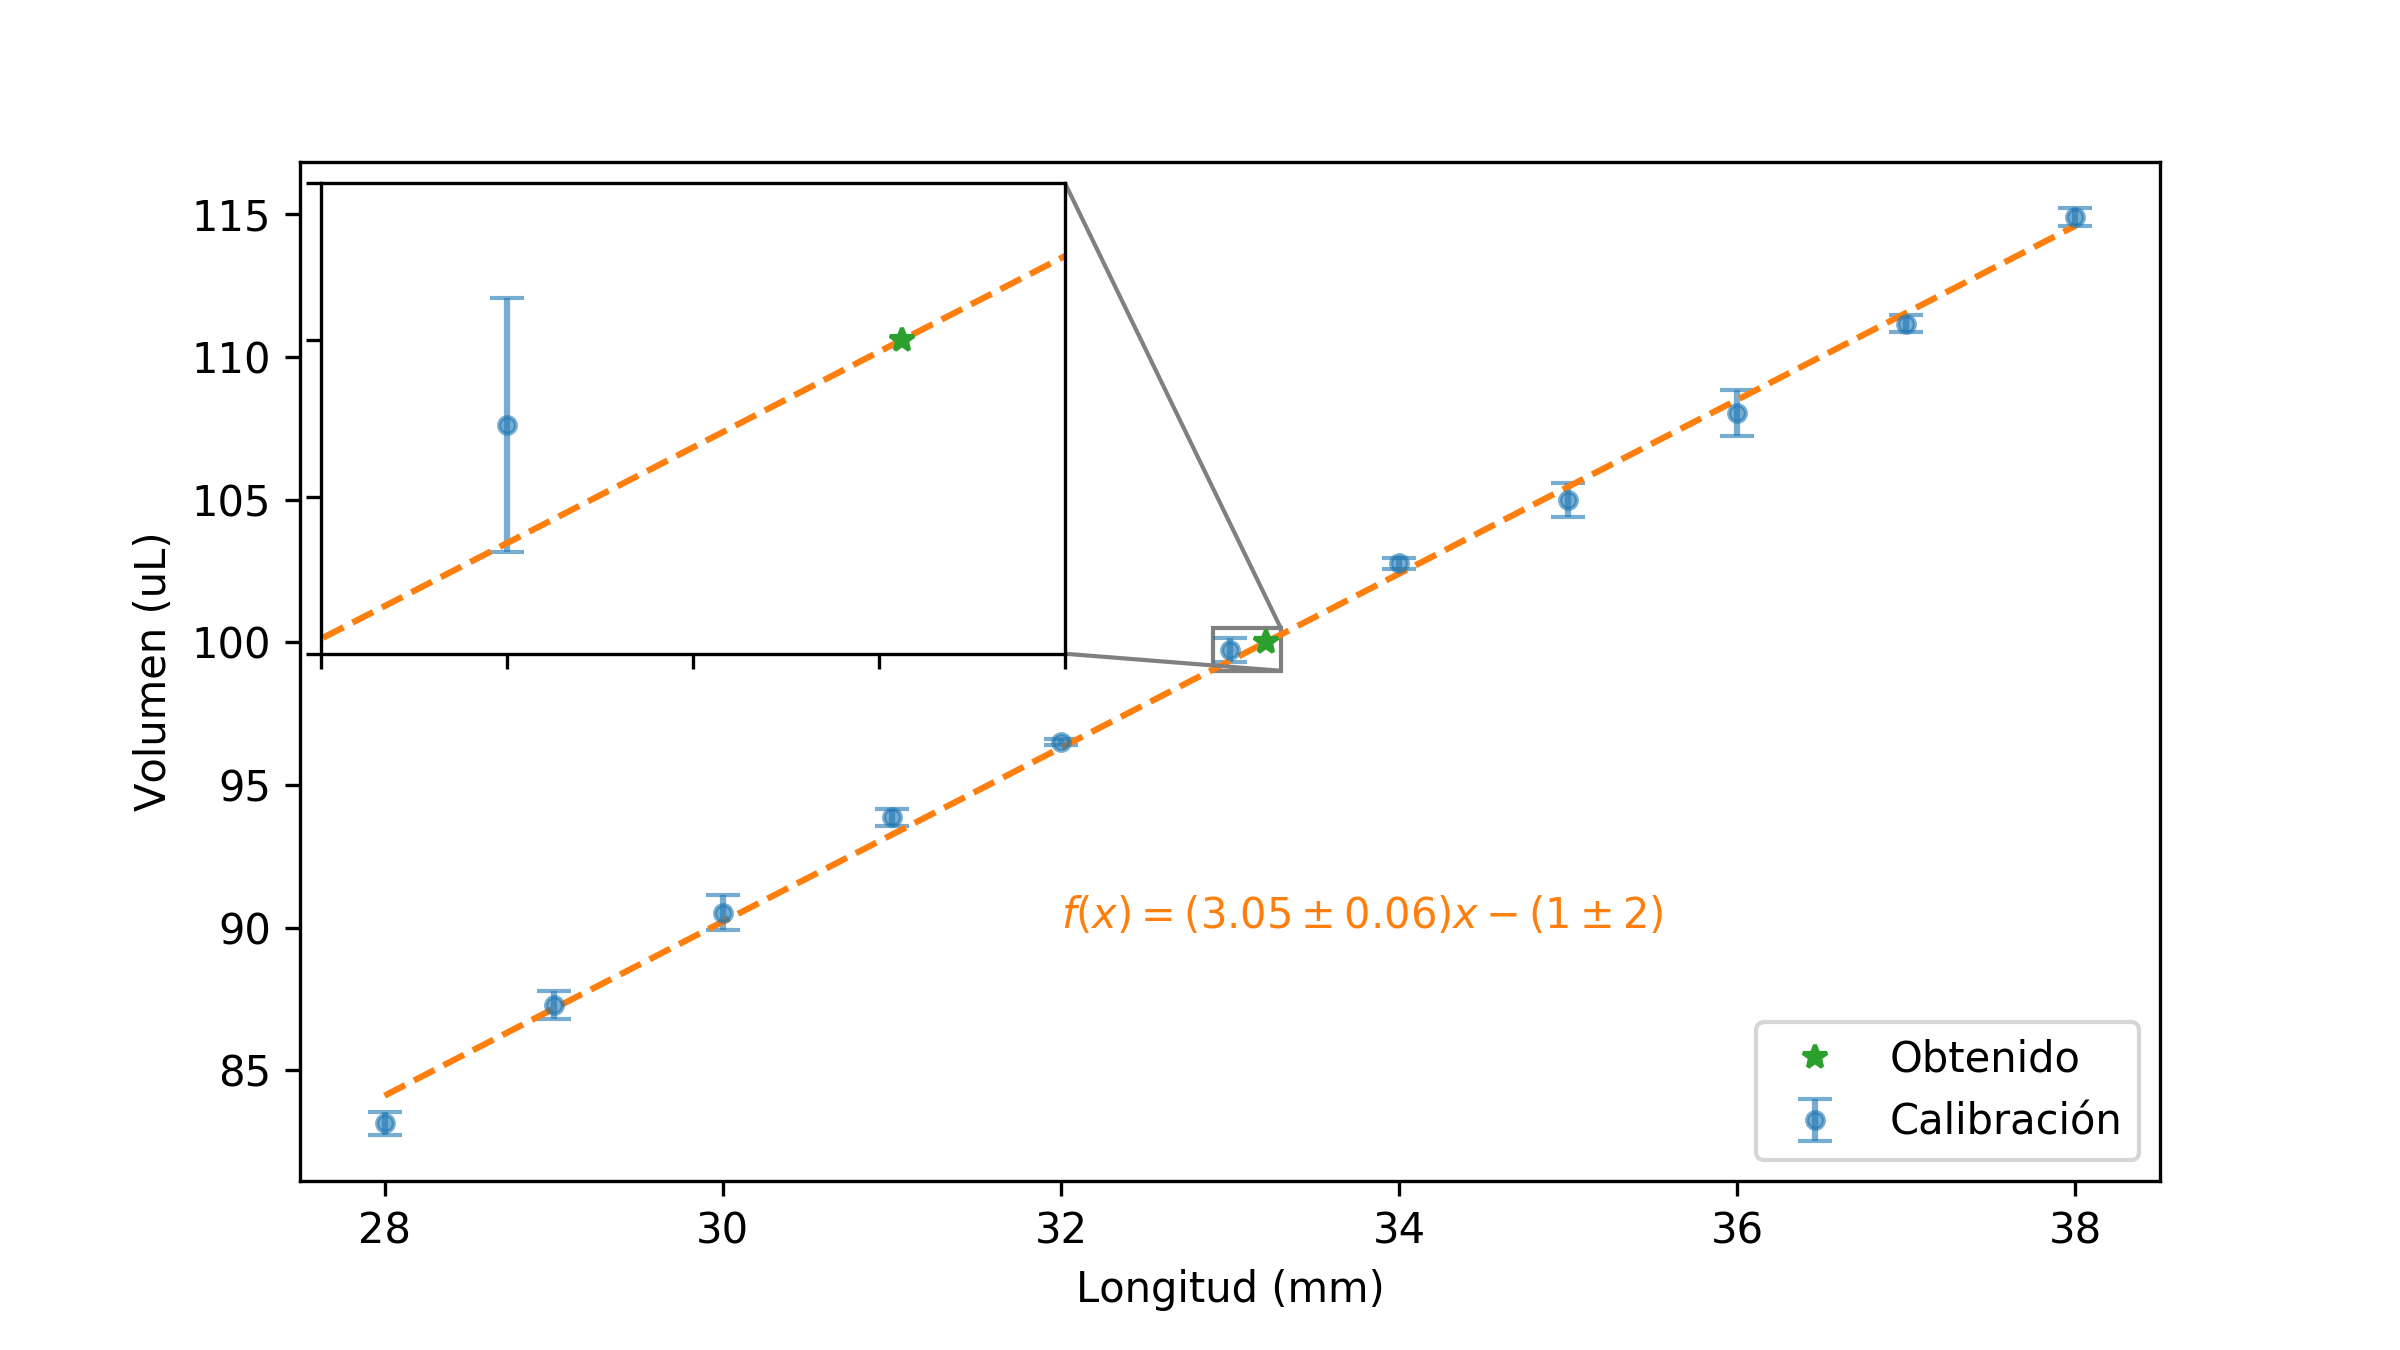
\includegraphics[width=\linewidth]{../Data/Syringe/syringe_cal.png}
			\caption{Curva de calibraci\'on de la jeringa usada.}
			\label{fig: syringeCal}
		\end{figure}
	
		Con el termómetro de mercurio usado en la calibración térmica de los sensores de temperatura se midió la temperatura del agua usada en la calibración de la jeringa, dando un valor de 17.7 $^\circ$C. El densimetro usado en la \autoref{sec: soluciones} fue configurado para realizar una lectura a esta misma temperatura, con lo cual se obtuvo un valor de densidad de 0.998679 g/cm$^3$. Con esta información es posible construir una curva que permite inferir la configuración a usar de la jeringa, esta curva junto con el valor escogido se muestran en la \autoref{fig: syringeCal}. Para un volumen de dispensación de 100 $\mu$L, se obtuvo una longitud de 33,213 mm.
		\newline
	
\section{Realizaci\'on del experimento}
	El m\'etodo experimental est\'a dividido en cuatro partes:
	\begin{enumerate}
		\item \textbf{Pause}: En la etapa inicial del experimento se busca medir el estado de la línea base por 120 minutos consecutivos.
		\item \textbf{Baseline}: Luego de tener datos sobre el estado sin perturbar del sistema, se realiza una calibración dinámica para realizar un ajuste fino de los parámetros de ganancia y nivel del cero de la señal. 
		\item \textbf{Pause:} En este punto se realiza una calibraci\'on est\'atica para confirmar que la calibraci\'on din\'amica fue correcta. Para esto, se aplican 300 $\mu$W sobre la celda por 30 minutos, posteriormente se retira la potencia y se esperan 50 minutos para la estabilizaci\'on de la linea base.
		\item \textbf{Main:} Una vez estabilizada la linea base, se realizan 30 inyecciones sucesivas con 10 minutos de espera entre cada inyecci\'on, la velocidad de inyecci\'on es de 50,018 $\mu/s$ y el volumen de inyecci\'on es de 51,185 $\mu$L.
	\end{enumerate}

	En la celda de medición fueron adicionados 1.6029 g de la solución de \ce{KHCO3} 0.17265 mM, y la jeringa fue cargada con 2.0 mL de la soluci\'on de HCl 0.2469 mM, y la temperatura del ba\~no t\'ermico se mantuvo en $25.05 \pm $ $^\circ$C a lo largo del experimento. 
\section{Resultados}


		